\documentclass{article}
\usepackage[utf8]{inputenc}
\usepackage{tikz}
\usetikzlibrary{mindmap}

\pagestyle{empty}
\begin{document}

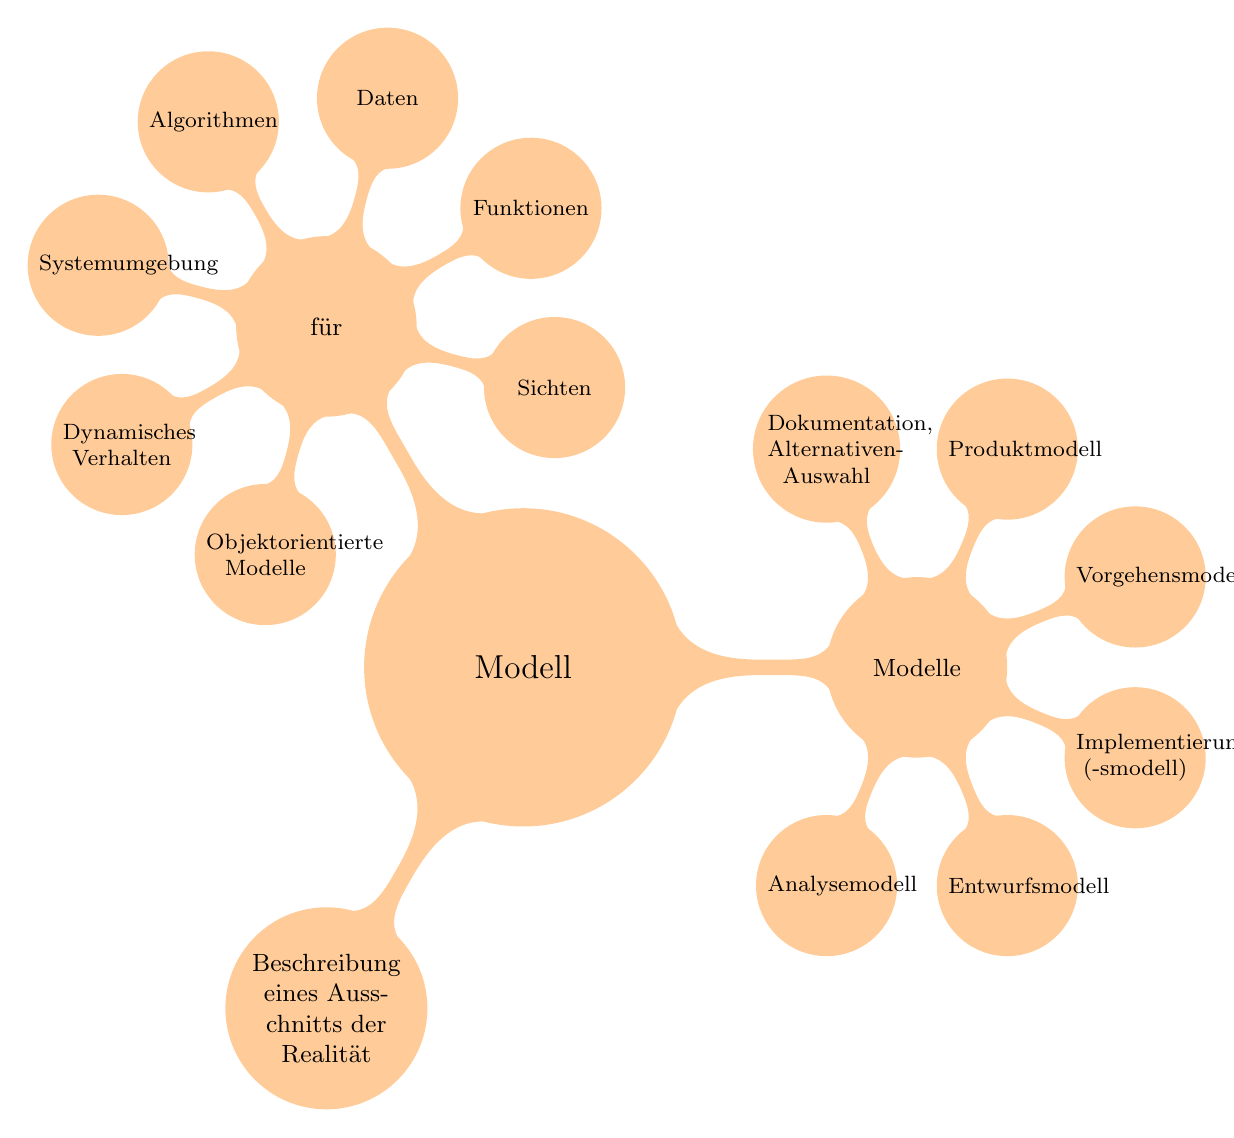
\begin{tikzpicture}[mindmap, grow cyclic, every node/.style=concept, concept color=orange!40,
        level 1/.append style={level distance=5cm,sibling angle=120},
        level 2/.append style={level distance=3cm,sibling angle=45}]

    \node{Modell}
    child { node {Beschreibung eines Ausschnitts der Realität}}
    child { node {Modelle}
            child { node {Analysemodell}}
            child { node {Entwurfsmodell}}
            child { node {Implementierung (-smodell)}}
            child { node {Vorgehensmodell}}
            child { node {Produktmodell}}
            child { node {Dokumentation, Alternativen-Auswahl}}
        }
    child { node {für}
            child { node {Sichten}}
            child { node {Funktionen}}
            child { node {Daten}}
            child { node {Algorithmen}}
            child { node {Systemumgebung}}
            child { node {Dynamisches Verhalten}}
            child { node {Objektorientierte Modelle}}
        };
\end{tikzpicture}


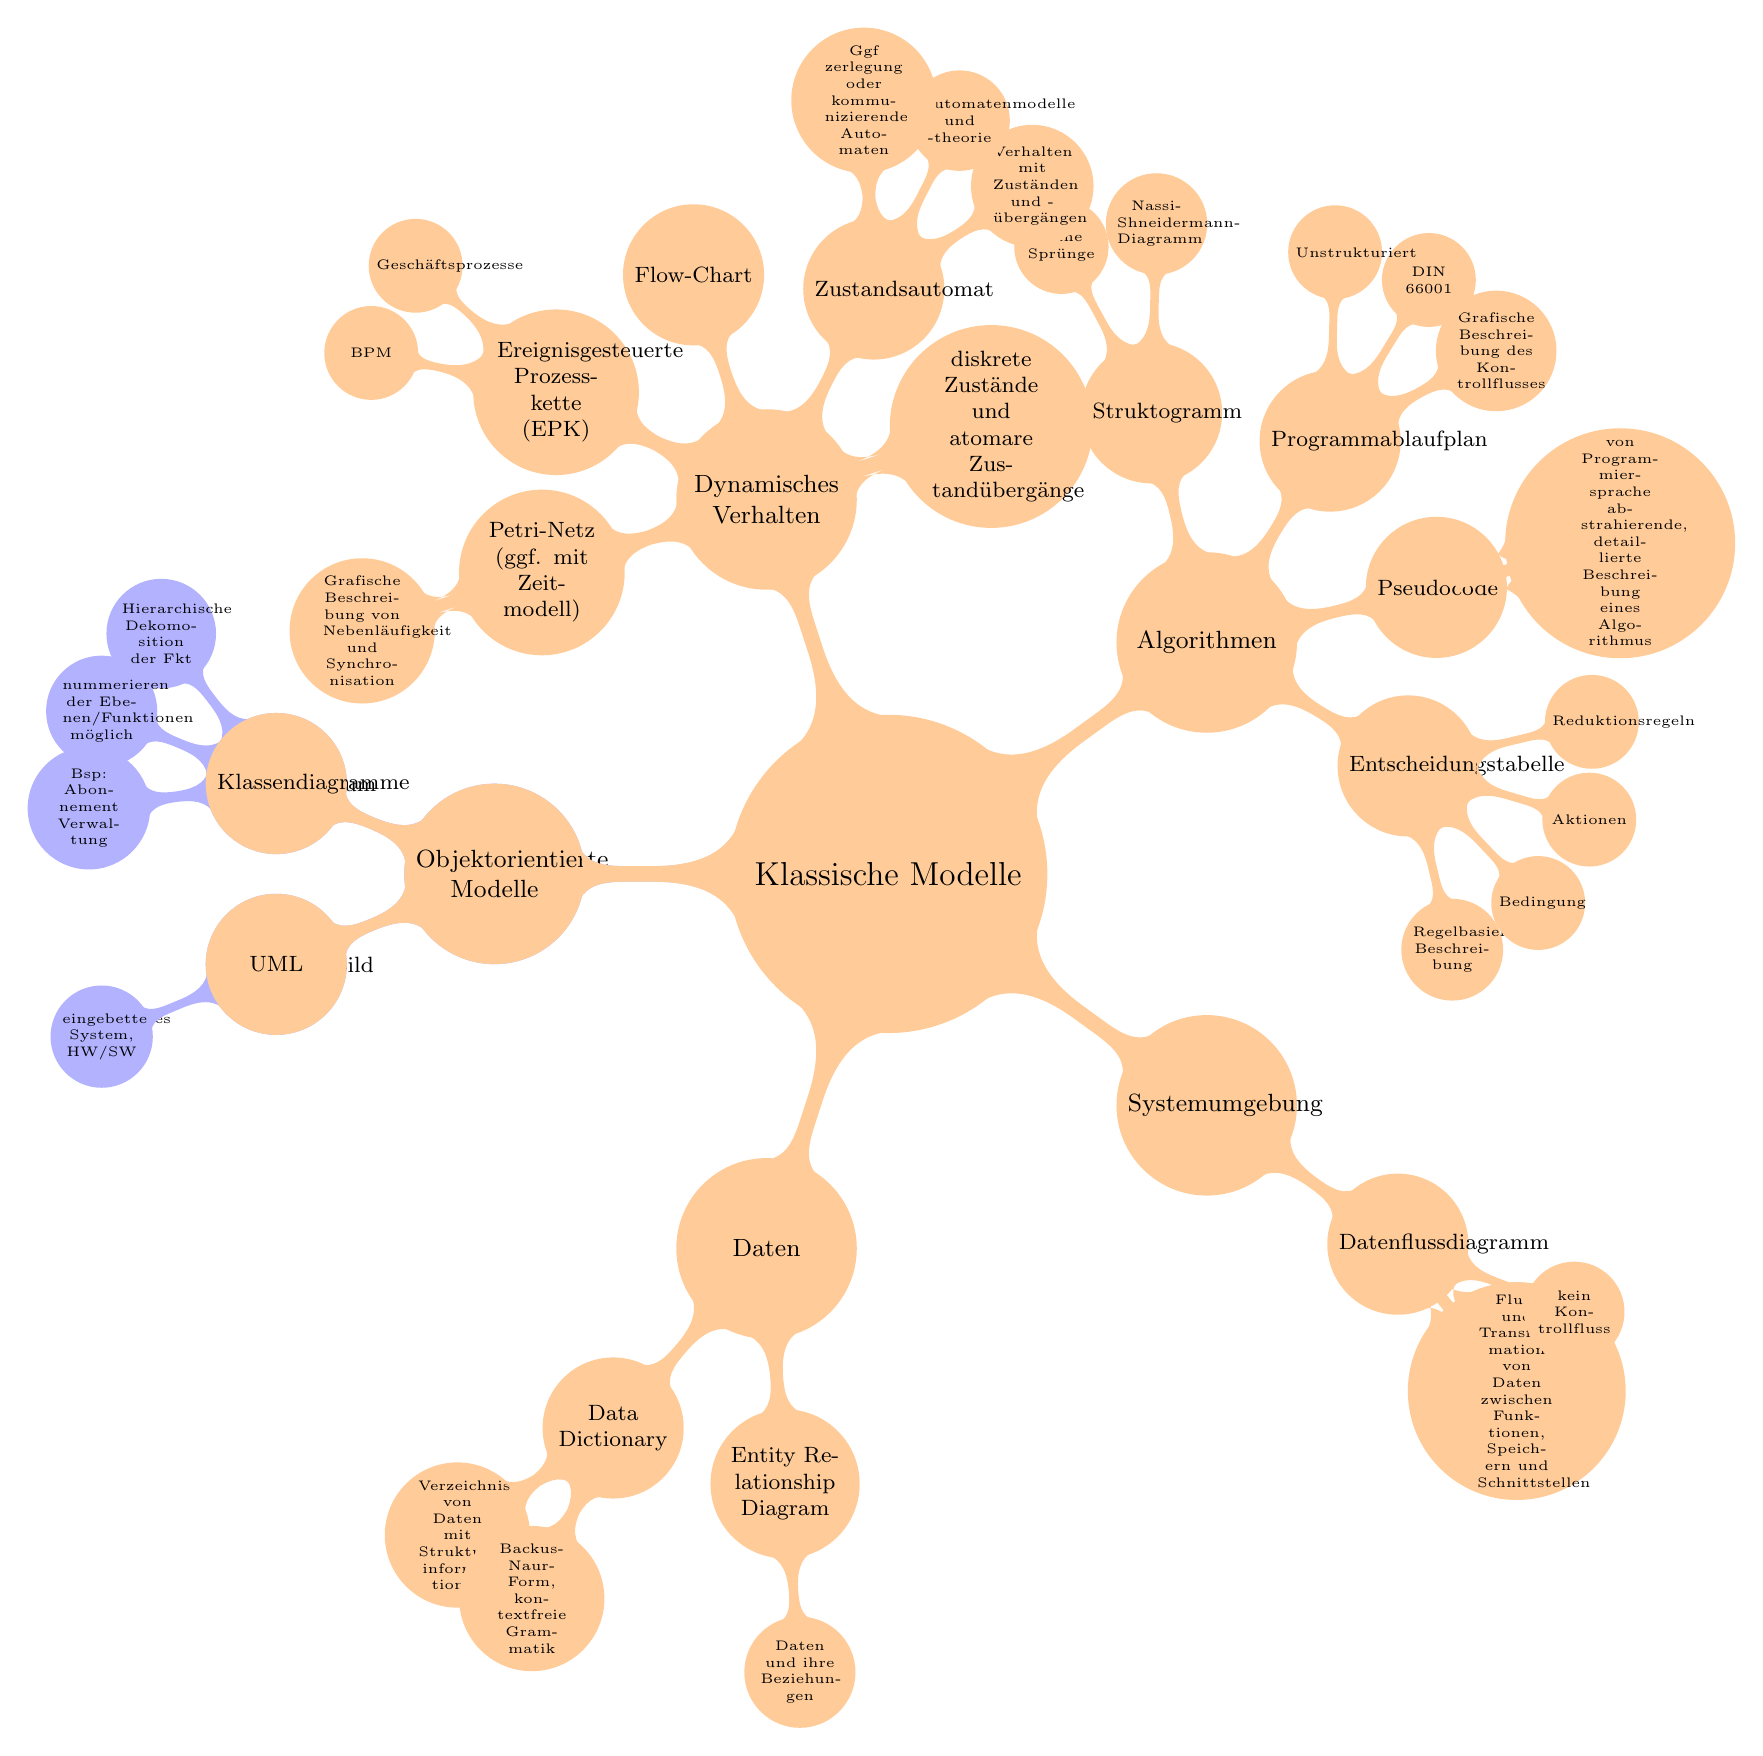
\begin{tikzpicture}[mindmap, grow cyclic, every node/.style=concept, concept color=orange!40,
        level 1/.append style={level distance=5cm,sibling angle=72},
        level 2/.append style={level distance=3cm,sibling angle=45}]

    \node{Klassische Modelle}
    child [concept color=blue!30]{ node {Funktionen}
            child { node {Funktionsbaum}
                    child { node {Hierarchische Dekomosition der Fkt}}
                    child { node {nummerieren der Ebenen/Funktionen möglich}}
                    child { node {Bsp: Abonnement Verwaltung}}
                }
            child { node {Blockschaltbild}
                    child { node {eingebettetes System, HW/SW}}
                }
        }
    child { node {Daten}
            child { node {Data Dictionary}
                    child { node {Verzeichnis von Daten mit Strukturinformationen}}
                    child { node {Backus-Naur-Form, kontextfreie Grammatik}}
                }
            child { node {Entity Relationship Diagram}
                    child { node {Daten und ihre Beziehungen}}
                }
        }
    child { node {Systemumgebung}
            child { node {Datenflussdiagramm}
                    child { node {Fluss und Transformation von Daten zwischen Funktionen, Speichern und Schnittstellen}}
                    child { node {kein Kontrollfluss}}
                }
        }
    child { node {Algorithmen}
            child { node {Entscheidungstabelle}
                    child { node {Regelbasierte Beschreibung}}
                    child { node {Bedingung}}
                    child { node {Aktionen}}
                    child { node {Reduktionsregeln}}
                }
            child { node {Pseudocode}
                    child { node {von Programmiersprache abstrahierende, detaillierte Beschreibung eines Algorithmus}}
                }
            child { node {Programmablaufplan}
                    child { node {Grafische Beschreibung des Kontrollflusses}}
                    child { node {DIN 66001}}
                    child { node {Unstrukturiert}}
                }
            child { node {Struktogramm}
                    child { node {Nassi-Shneidermann-Diagramm}}
                    child { node {keine Sprünge}}
                }
        }
    child { node {Dynamisches Verhalten}
                child { node {diskrete Zustände und atomare Zustandübergänge}}
            child { node {Zustandsautomat}
                    child { node {Verhalten mit Zuständen und -übergängen}}
                    child { node {Automatenmodelle und -theorie}}
                    child { node {Ggf zerlegung oder kommunizierende Automaten}}
                }
            child { node {Flow-Chart}}
            child { node {Ereignisgesteuerte Prozesskette (EPK)}
                    child { node {Geschäftsprozesse}}
                    child { node {BPM}}
                }
            child { node {Petri-Netz (ggf. mit Zeitmodell)}
                    child { node {Grafische Beschreibung von Nebenläufigkeit und Synchronisation}}
                }
        }
    child { node {Objektorientierte Modelle}
            child { node {Klassendiagramme}}
            child { node {UML}}
        };
\end{tikzpicture}

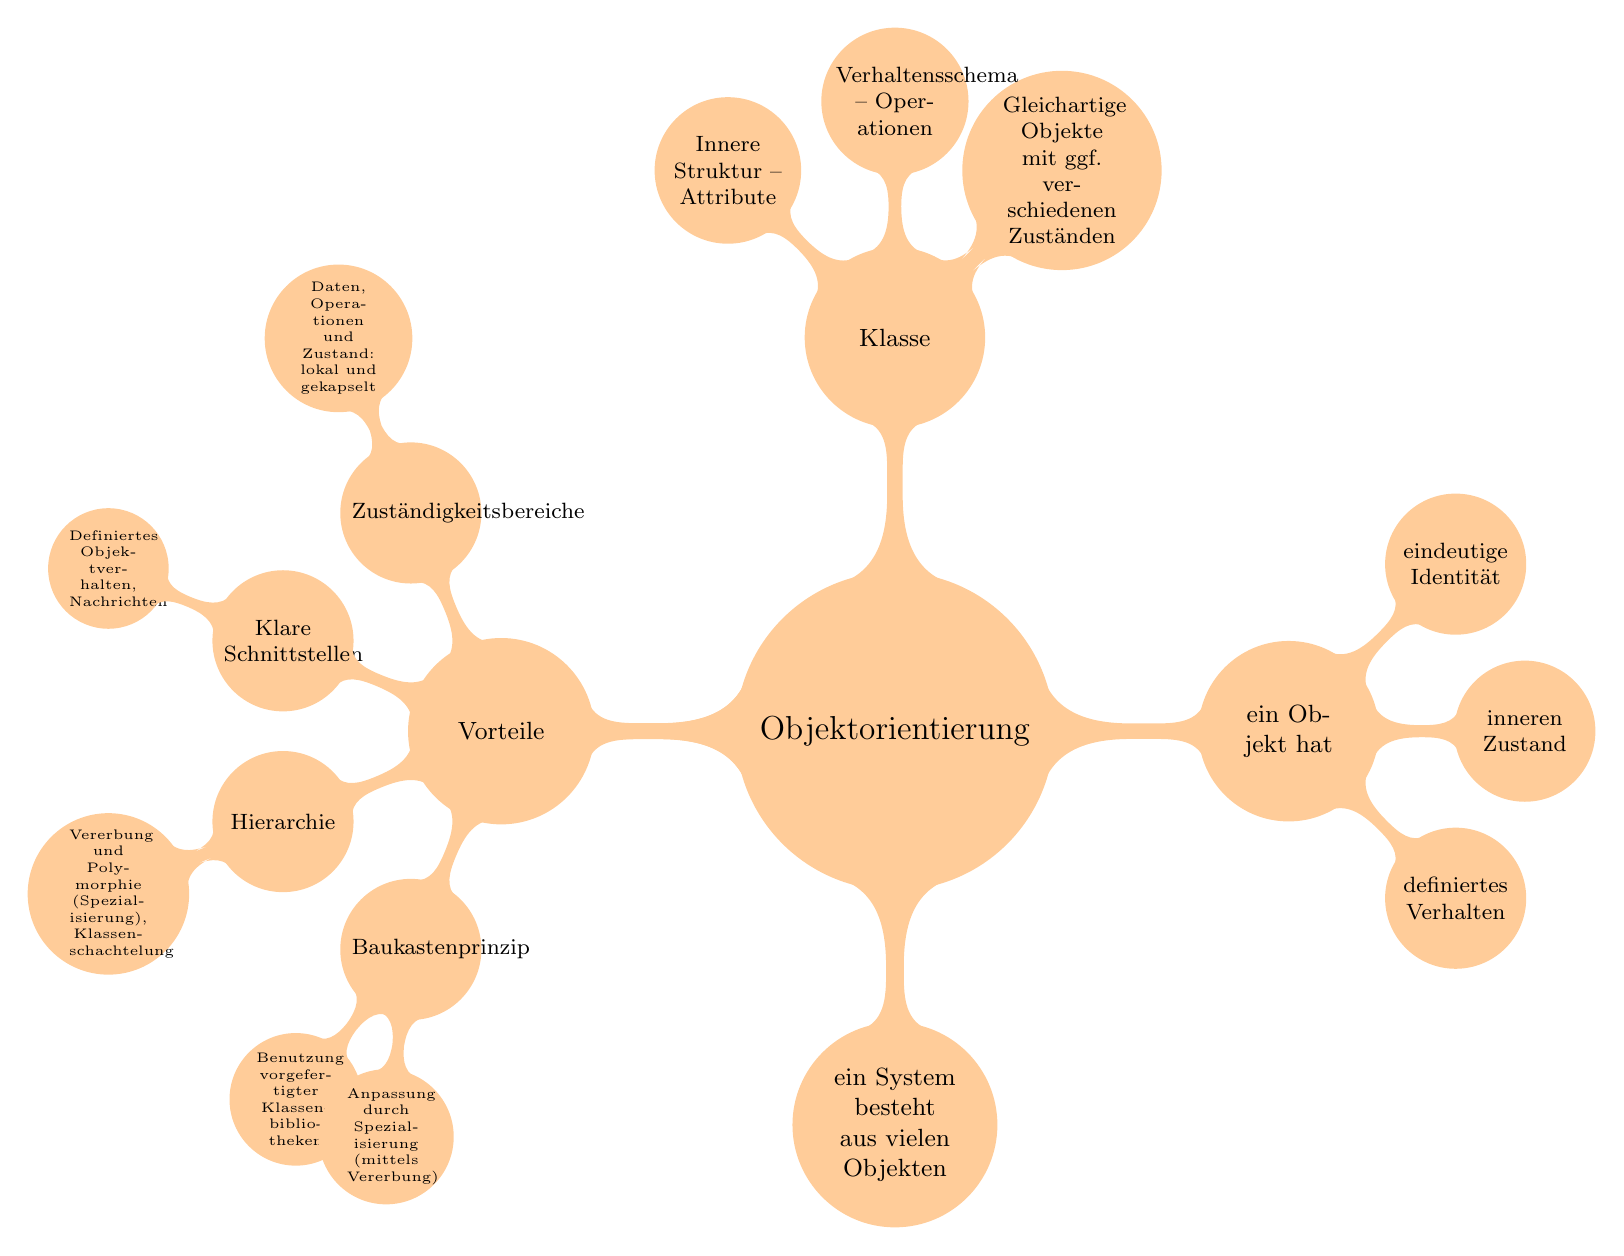
\begin{tikzpicture}[mindmap, grow cyclic, every node/.style=concept, concept color=orange!40,
        level 1/.append style={level distance=5cm,sibling angle=90},
        level 2/.append style={level distance=3cm,sibling angle=45}]

    \node{Objektorientierung}
    child { node {Grundprinzip: Teile und Herrsche}}
    child { node {ein System besteht aus vielen Objekten}}
    child { node {ein Objekt hat}
            child { node {definiertes Verhalten}}
            child { node {inneren Zustand}}
            child { node {eindeutige Identität}}
        }
    child { node {Klasse}
            child { node {Gleichartige Objekte mit ggf. verschiedenen Zuständen}}
            child { node {Verhaltensschema – Operationen}}
            child { node {Innere Struktur – Attribute}}
        }
    child { node {Vorteile}
            child { node {Zuständigkeitsbereiche}
                    child { node {Daten, Operationen und Zustand: lokal und gekapselt}}
                }
            child { node {Klare Schnittstellen}
                    child { node {Definiertes Objektverhalten, Nachrichten}}
                }
            child { node {Hierarchie}
                    child { node {Vererbung und Polymorphie (Spezialisierung), Klassenschachtelung}}
                }
            child { node {Baukastenprinzip}
                    child { node {Benutzung vorgefertigter Klassenbibliotheken}}
                    child { node {Anpassung durch Spezialisierung (mittels Vererbung)}}
                }
        };
\end{tikzpicture}

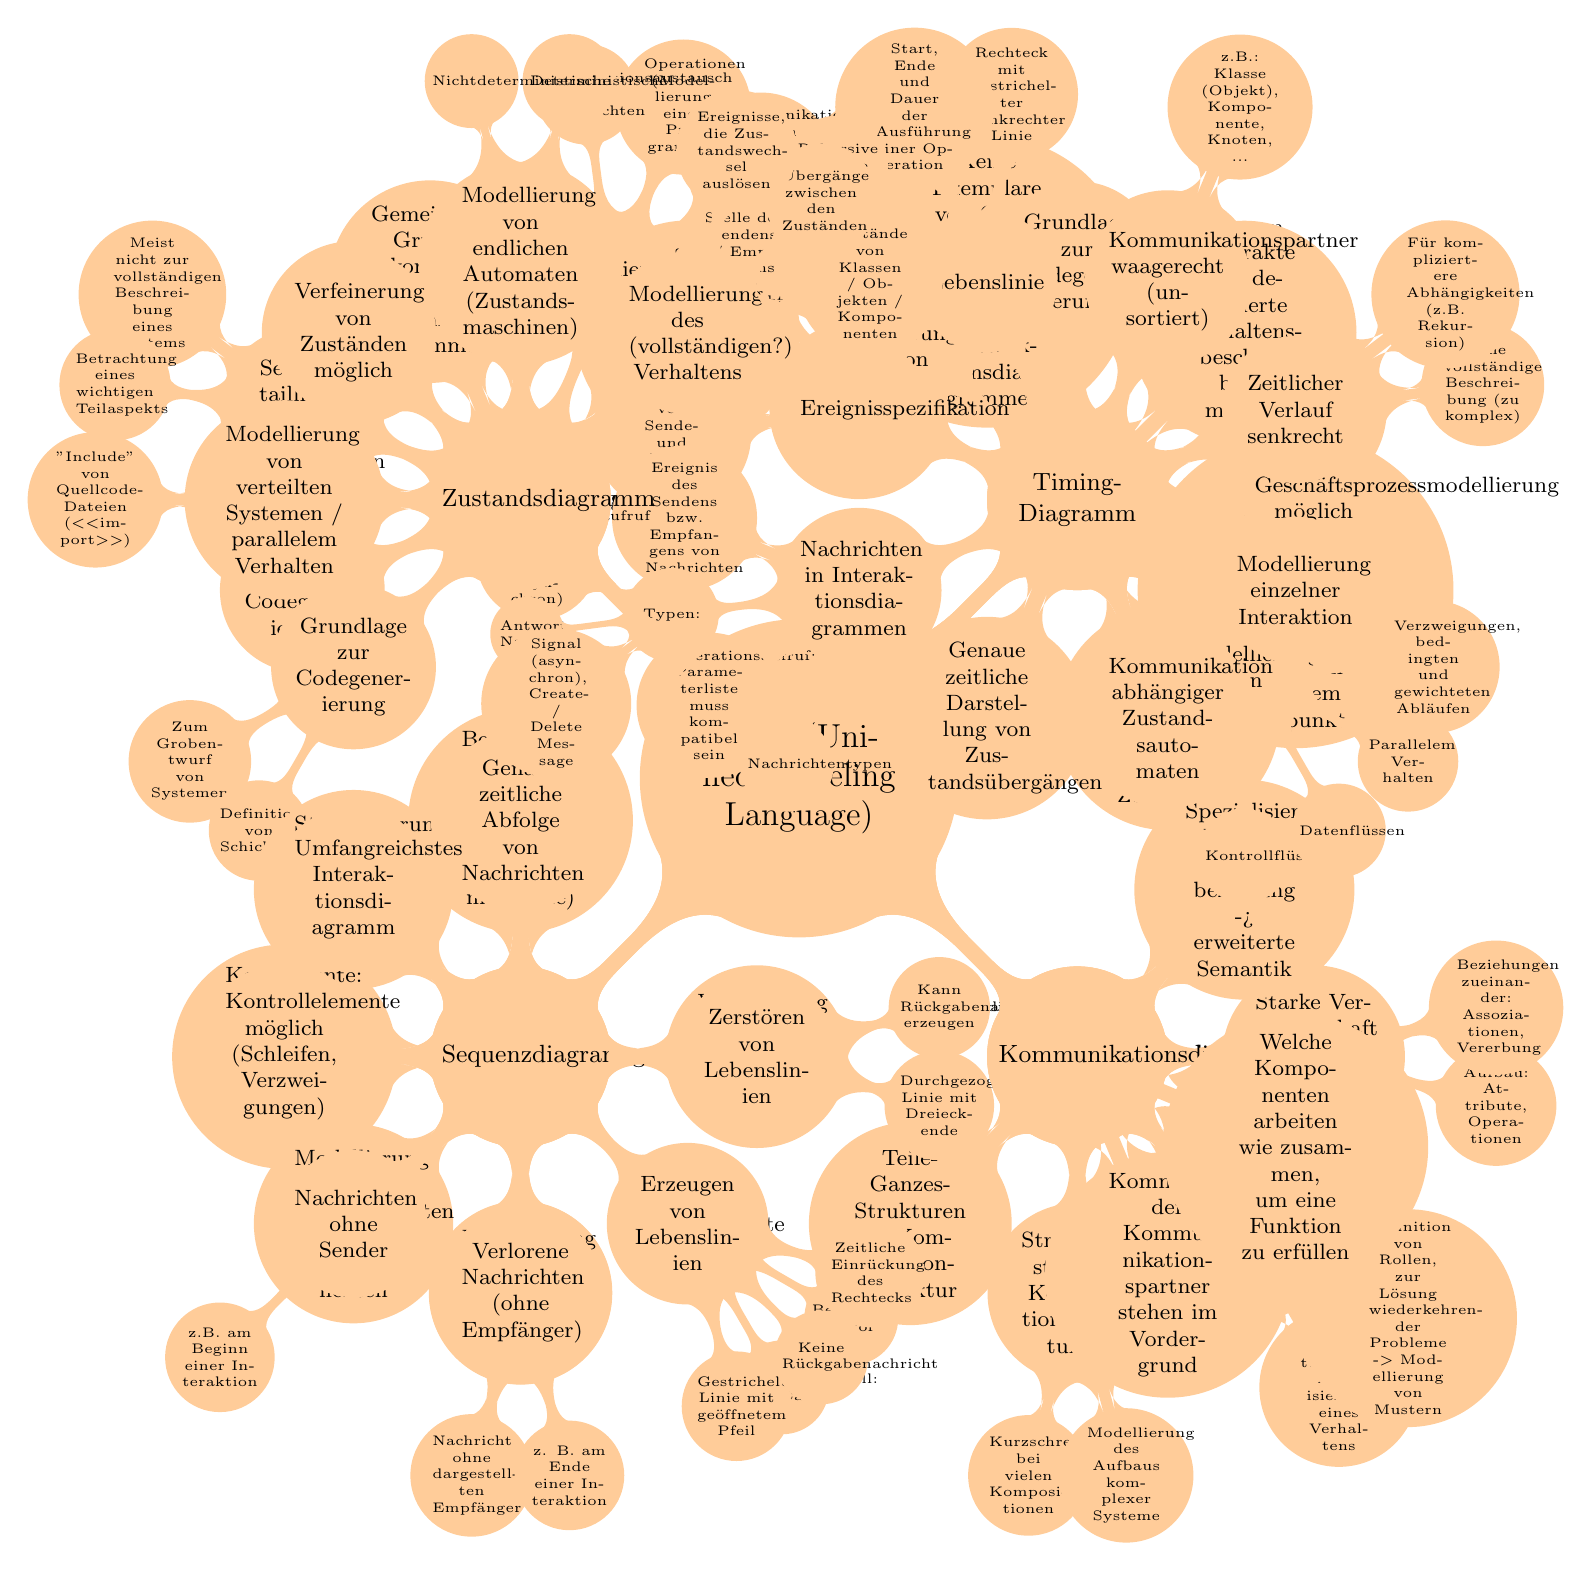
\begin{tikzpicture}[mindmap, grow cyclic, every node/.style=concept, concept color=orange!40,
        level 1/.append style={level distance=5cm,sibling angle=90},
        level 2/.append style={level distance=3cm,sibling angle=45}]

    \node{UML (Unified Modeling Language)}
    child { node {Use-Case-Diagramm}
            child { node {Beschreiben Systemfunktion aus Benutzersicht (Was, nicht Wie)}}
            child { node {Erste Anforderungsspezifikation (requirements)}}
            child { node {Planbare Einheiten als Inkremente für die Entwicklung}}
            child { node {Keine Modellierung eines Ablaufs!}}
            child { node {Erstellen von Testfällen (test case generation)}}
            child { node {Grundelemente}
                    child { node {Anwendungsfall: Use Case}}
                    child { node {Beteiligte: Aktor}}
                }
            child { node {Verfeinerung mittels Use-Case-Realisierung notwendig}
                    child { node {Textuelle Beschreibung}}
                    child { node {Verhaltensdiagramme}}
                }
        }
    child { node {Klassendiagramm}
            child { node {Modellierung der Struktur (Aufbau) eines Systems}}
            child { node {Modellierung von statischen Aspekten}}
            child { node {Modellierung der Struktur von Daten}}
            child { node {Klasse im Mittelpunkt}
                    child { node {Aufbau: Attribute, Operationen}}
                    child { node {Beziehungen zueinander: Assoziationen, Vererbung}}
                }
            child { node {Verbreitetstes und bekanntestes Diagramm der UML}}
        }
    child { node {Objektdiagramm}
            child { node {Struktur des Systems zur Laufzeit zu einem Zeitpunkt}}
            child { node {Tatsächliche Zusammenhänge und Belegungen von Attributen von Objekten zu einem Zeitpunkt}}
            child { node {Eine detaillierte Sicht auf einen Aspekt}
                    child { node {Keine vollständige Beschreibung (zu komplex)}}
                    child { node {Für kompliziertere Abhängigkeiten (z.B. Rekursion)}}
                }
            child { node {Objektdiagramm für alle Arten von Exemplaren}
                    child { node {z.B.: Klasse (Objekt), Komponente, Knoten, ...}}
                }
            child { node {Keine Exemplare von Operationen -> Ablauf -> Verhaltensdiagramme / Interaktionsdiagramme}}
            child { node {Kein Verlauf der Wertebelegung über die Zeit}}
        }
    child { node {Paketdiagramm}
            child { node {Gliederung (Strukturierung) des Systems in Teile (Pakete)}}
            child { node {Zuordnung von Elementen zu einem Paket}}
            child { node {Bildung von Hierarchien (Enthält-Beziehung)}}
            child { node {Abhängigkeiten zwischen den Paketen}
                    child { node {"Include" von Quellcode-Dateien (<<import>>)}}
                }
            child { node {Anwendung:}
                    child { node {Zum Grobentwurf von Systemen}}
                    child { node {Definition von Schichten}}
                }
        }
    child { node {Komponentendiagramm}
            child { node {Strukturierung des Systems durch Komponenten}}
            child { node {Komponente: Modulare, austauschbare Einheit (Substitution)}}
            child { node {Modellierung der Abhängigkeiten zwischen Komponenten}}
            child { node {Modellierung der inneren Struktur von Komponenten}}
            child { node {Definition von Schnittstellen}}
        }
    child { node {Kompositionsstrukturdiagramm}
            child { node {Teile-Ganzes-Strukturen -> Kompositionsstruktur}}
            child { node {Strukturell statische Kompositionsstrukturen:}
                    child { node {Kurzschreibweise bei vielen Kompositionen}}
                    child { node {Modellierung des Aufbaus komplexer Systeme}}
                }
            child { node {Strukturell dynamische Kompositionsstrukturen:}
                    child { node {Notwendige Strukturen zur Realisierung eines Verhaltens}}
                    child { node {Definition von Rollen, zur Lösung wiederkehrender Probleme -> Modellierung von Mustern}}
                }
            child { node {Starke Verwandtschaft mit dem Klassendiagramm}}
            child { node {Spezialisierte Kompositionsbeziehung -> erweiterte Semantik}}
        }
    child { node {Aktivitätsdiagramm}
            child { node {Modellierung von}
                    child { node {Kontrollflüssen}}
                    child { node {Datenflüssen}}
                    child { node {Parallelem Verhalten}}
                    child { node {Verzweigungen, bedingten und gewichteten Abläufen}}
                }
            child { node {Geschäftsprozessmodellierung möglich}}
            child { node {Abstrakte und detaillierte Verhaltensbeschreibung möglich}}
            child { node {Grundlage zur Codegenerierung}}
            child { node {Zur Verfeinerung von}
                    child { node {Use-Cases}}
                    child { node {Operationen / Interaktionen}}
                    child { node {anderen Aktionen und Aktivitäten}}
                }
        }
    child { node {Interaktionsdiagramme}
            child { node {Modellierung von}
                    child { node {Kommunikation zwischen Kommunikationspartnern (Lebenslinie)}}
                    child { node {Operationen (Modellierung eines Programms)}}
                    child { node {Informationsaustausch / Nachrichten}}
                }
            child { node {Gemeinsames Grundkonzept der Interaktionsdiagramme}}
            child { node {Sehr detaillierte Diagramme}
                    child { node {Meist nicht zur vollständigen Beschreibung eines Systems}}
                    child { node {Betrachtung eines wichtigen Teilaspekts}}
                }
            child { node {Grundlage zur Codegenerierung}}
        }
    child { node {Sequenzdiagramm}
            child { node {Genaue zeitliche Abfolge von Nachrichten}}
            child { node {Umfangreichstes Interaktionsdiagramm}}
            child { node {Kontrollelemente möglich (Schleifen, Verzweigungen)}}
            child { node {Nachrichten ohne Sender}
                    child { node {z.B. am Beginn einer Interaktion}}
                }
            child { node {Verlorene Nachrichten (ohne Empfänger)}
                    child { node {Nachricht ohne dargestellten Empfänger}}
                    child { node {z. B. am Ende einer Interaktion}}
                }
            child { node {Erzeugen von Lebenslinien}
                    child { node {Gestrichelte Linie mit geöffnetem Pfeil}}
                    child { node {Keine Rückgabenachricht}}
                    child { node {Zeitliche Einrückung des Rechtecks}}
                }
            child { node {Zerstören von Lebenslinien}
                    child { node {Durchgezogene Linie mit Dreieckende}}
                    child { node {Kann Rückgabenachricht erzeugen}}
                }
        }
    child { node {Kommunikationsdiagramm}
            child { node {Kommunikationsbeziehungen der Kommunikationspartner stehen im Vordergrund}}
            child { node {Welche Komponenten arbeiten wie zusammen, um eine Funktion zu erfüllen}}
        }
    child { node {Timing-Diagramm}
            child { node {Genaue zeitliche Darstellung von Zustandsübergängen}}
            child { node {Kommunikation abhängiger Zustandsautomaten}}
            child { node {Modellierung einzelner Interaktion}}
            child { node {Zeitlicher Verlauf senkrecht}}
            child { node {Kommunikationspartner waagerecht (unsortiert)}}
            child { node {Lebenslinie}
                    child { node {Rechteck mit gestrichelter senkrechter Linie}}
                    child { node {Start, Ende und Dauer der Ausführung einer Operation}}
                    child { node {Rekursive Aufrufe möglich}}
                }
            child { node {Ereignisspezifikation}
                    child { node {Stelle des Sendens / Empfangens der Nachricht}}
                    child { node {Definition der Reihenfolge des Auftretens}}
                    child { node {Trace: Folge von Sende-und Empfangsereignissen}}
                }
            child { node {Nachrichten in Interaktionsdiagrammen}
                    child { node {Ereignis des Sendens bzw. Empfangens von Nachrichten}}
                    child { node {Typen:}
                            child { node {Operationsaufruf (synchron / asynchron)}}
                            child { node {Antwort Nachricht}}
                            child { node {Signal (asynchron), Create-/ Delete Message}}
                        }
                    child { node {Operationsaufruf: Parameterliste muss kompatibel sein}}
                    child { node {Nachrichtentypen}}
                }
        }
    child { node {Zustandsdiagramm}
            child { node {Modellierung des (vollständigen?) Verhaltens}
                    child { node {Zustände von Klassen / Objekten / Komponenten}}
                    child { node {Übergänge zwischen den Zuständen}}
                    child { node {Ereignisse, die Zustandswechsel auslösen}}
                }
            child { node {Modellierung von endlichen Automaten (Zustandsmaschinen)}
                    child { node {Deterministische}}
                    child { node {Nichtdeterministische}}
                }
            child { node {Verfeinerung von Zuständen möglich}}
            child { node {Modellierung von verteilten Systemen / parallelem Verhalten}}
            child { node {Grundlage zur Codegenerierung}}
        };
\end{tikzpicture}

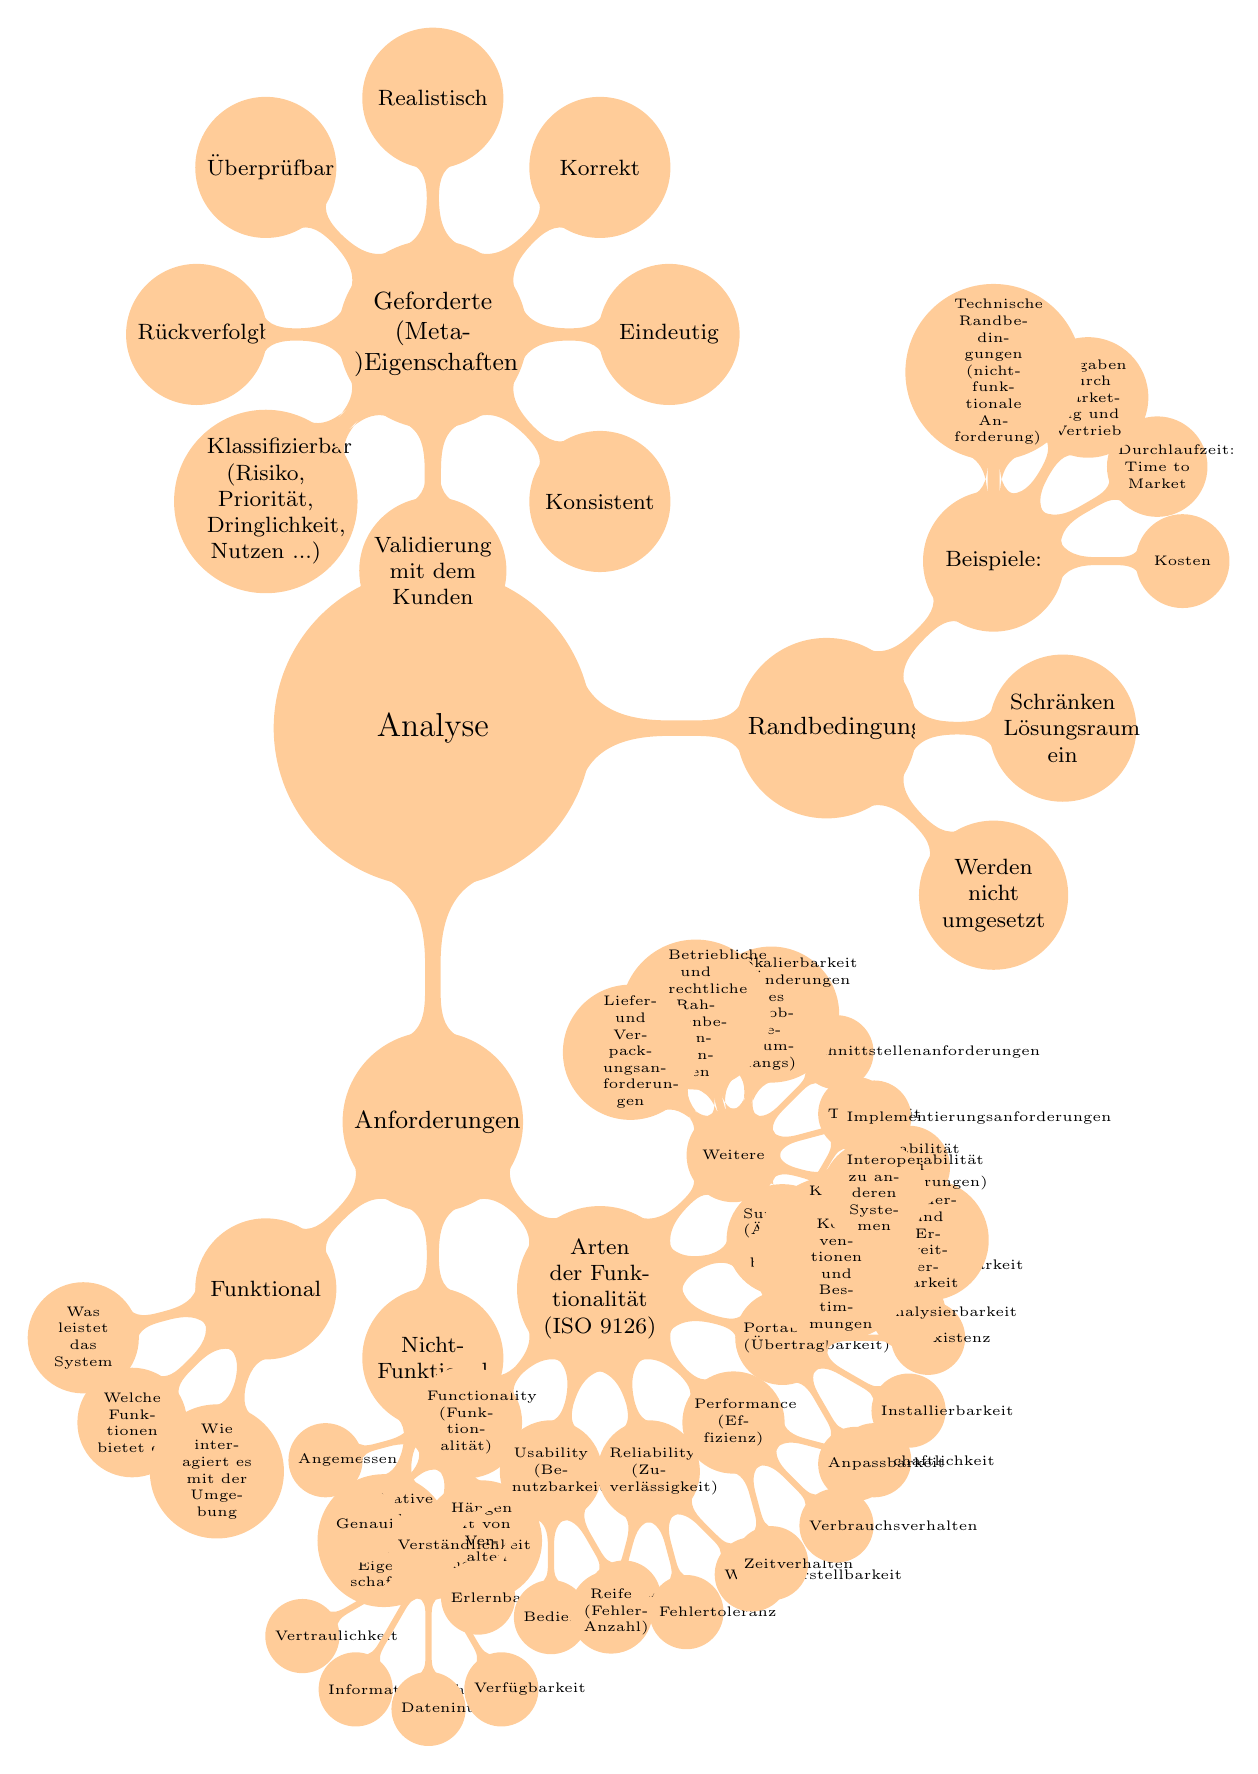
\begin{tikzpicture}[mindmap, grow cyclic, every node/.style=concept, concept color=orange!40,
    level 1/.append style={level distance=5cm,sibling angle=90},
    level 2/.append style={level distance=3cm,sibling angle=45}]

\node{Analyse}
child { node {Anforderungen}
    child { node {Funktional}
        child { node {Was leistet das System}}
        child { node {Welche Funktionen bietet es}}
        child { node {Wie interagiert es mit der Umgebung}}
    }
    child { node {Nicht-Funktional}
        child { node {qualitative oder quantitative Eigenschaften}}
        child { node {Hängen oft von Verhalten ab}}
    }
    child { node {Arten der Funktionalität (ISO 9126)}
        child { node {Functionality (Funktionalität)}
            child { node {Angemessen}}
            child { node {Genauigkeit}}
            child { node {Sicherheit}
                child { node {Vertraulichkeit}}
                child { node {Informationssicherheit}}
                child { node {Datenintegrität}}
                child { node {Verfügbarkeit}}
            }
        }
        child { node {Usability (Benutzbarkeit)}
            child { node {Verständlichkeit}}
            child { node {Erlernbarkeit}}
            child { node {Bedienbarkeit}}
            child { node {Attraktivität}}
        }
        child { node {Reliability (Zuverlässigkeit)}
            child { node {Reife (Fehler-Anzahl)}}
            child { node {Fehlertoleranz}}
            child { node {Wiederherstellbarkeit}}
        }
        child { node {Performance (Effizienz)}
            child { node {Zeitverhalten}}
            child { node {Verbrauchsverhalten}}
            child { node {Wirtschaftlichkeit}}
        }
        child { node {Portability (Übertragbarkeit)}
            child { node {Anpassbarkeit}}
            child { node {Installierbarkeit}}
            child { node {Koexistenz}}
            child { node {Austauschbarkeit}}
        }
        child { node {Supportability (Änderbarkeit/ Wartbarkeit)}
            child { node {Analysierbarkeit}}
            child { node {Änder-und Erweiterbarkeit}}
            child { node {Stabilität (bei Änderungen)}}
            child { node {Testbarkeit}}
        }
        child { node {Weitere}
            child { node {Konformität zu Konventionen und Bestimmungen}}
            child { node {Interoperabilität zu anderen Systemen}}
            child { node {Implementierungsanforderungen}}
            child { node {Schnittstellenanforderungen}}
            child { node {Skalierbarkeit (Änderungen des Problemumfangs)}}
            child { node {Betriebliche und rechtliche Rahmenbedingungen}}
            child { node {Liefer-und Verpackungsanforderungen}}
        }
    }
}
child { node {Randbedingungen}
    child { node {Werden nicht umgesetzt}}
    child { node {Schränken Lösungsraum ein}}
    child { node {Beispiele:}
    child { node {Kosten}}
    child { node {Durchlaufzeit: Time to Market}}
    child { node {Vorgaben durch Marketing und Vertrieb}}
    child { node {Technische Randbedingungen (nichtfunktionale Anforderung)}}
    }
}
child { node {Geforderte (Meta-)Eigenschaften}
    child { node {Vollständig}}
    child { node {Konsistent}}
    child { node {Eindeutig}}
    child { node {Korrekt}}
    child { node {Realistisch}}
    child { node {Überprüfbar}}
    child { node {Rückverfolgbar}}
    child { node {Klassifizierbar (Risiko, Priorität, Dringlichkeit, Nutzen ...)}}
    child { node {Validierung mit dem Kunden}}
}
;
\end{tikzpicture}

\end{document}
